\section{定位方程}
\subsection{单点定位方程}
\begin{frame}{定位方程模型}
    \begin{itemize}
        \item 测距码方程组
        \begin{align*}
            \tilde \rho _ R ^ { S _ i } &= \textcolor{red}{ \rho _ R ^ { S _ i } } - c \textcolor{red}{ \delta t _ R } \\
            &+ c \delta t _ { S _ i } - V _ { \mathrm{ iono }, S _ i } ^ R - V _ { \mathrm{ trop }, S _ i } ^ R, \
            i = 1, \ldots, n _ s
        \end{align*}
        \item 载波相位方程组
        \begin{align*}
            \lambda \tilde \varphi _ R ^ { S _ i } &= \textcolor{red}{ \rho _ R ^ { S _ i } } - c
            \textcolor{red}{ \delta t _ R } - \lambda \textcolor{red}{ N _ R ^ { S _ i } } \\
            &+ c \delta t _ { S _ i } - V _ { \mathrm{ iono }, S _ i } ^ R - V _ { \mathrm{ trop }, S _ i } ^ R, \
            i = 1, \ldots, n _ s
        \end{align*}
    \end{itemize}
\end{frame}

\subsection{差分定位}
\begin{frame}{差分模型图例}
    \begin{figure}
        \centering
        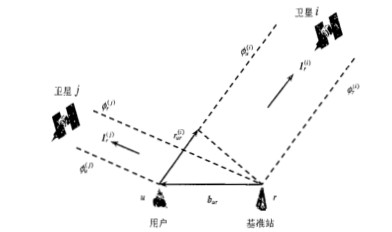
\includegraphics[width = .7\textwidth]{pic/single_double_diff.jpg}
        \caption{差分模型图例}
        \label{fig:single_double_diff}
    \end{figure}
\end{frame}

\begin{frame}{单差定位方程}
    \begin{itemize}
        \item 基准站位置$B\left( x ^ B, y ^ B, z ^ B \right)$
        \begin{align*}
            \lambda \tilde \varphi _ B ^ { S _ i } &= \rho _ B ^ { S _ i } - c \delta t _ B - \lambda N _ B ^ { S _ i }
            + c \delta t _ { S _ i } - V _ { \mathrm{ iono }, S _ i } ^ B - V _ { \mathrm{ trop }, S _ i } ^ B
        \end{align*}
        \item 单差定位方程
        \begin{align*}
            \lambda \tilde \varphi _ { BR } ^ { S _ i } &= \rho _ { BR } ^ { S _ i } - c \delta t _ { BR } - \lambda N _ { BR } ^ { S _ i } \\
            &- V _ { \mathrm{ iono }, S _ i } ^ { BR } - V _ { \mathrm{ trop }, S _ i } ^ { BR }, \ i = 1, \ldots, n _ s
        \end{align*}
        \item 记号说明
        \begin{align*}
            \star _ { BR } &= \star _ R - \star _ B
        \end{align*}
    \end{itemize}
\end{frame}

\begin{frame}{双差定位方程}
    \begin{itemize}
        \item 卫星$S _ j$单差定位方程
        \begin{align*}
            \lambda \tilde \varphi _ { BR } ^ { S _ j } &= \rho _ { BR } ^ { S _ j } - c \delta t _ { BR } - \lambda N _ { BR } ^ { S _ j } \\
            &- V _ { \mathrm{ iono }, S _ j } ^ { BR } - V _ { \mathrm{ trop }, S _ j } ^ { BR }, \ j = 1, \ldots, n _ s
        \end{align*}
        \item 双差定位方程
        \begin{align*}
            \lambda \tilde \varphi _ { BR } ^ { S _ { ij } } &= \rho _ { BR } ^ { S _ { ij } } - \lambda N _ { BR } ^ { S _ { ij } } \\
            &- V _ { \mathrm{ iono }, S _ { ij } } ^ { BR } - V _ { \mathrm{ trop }, S _ { ij } } ^ { BR }, \ i \ne j, i, j = 1, \ldots, n _ s
        \end{align*}
        \item 记号说明
        \begin{align*}
            \star _ { ij } &= \star _ i - \star _ j
        \end{align*}
    \end{itemize}
\end{frame}

\section{定位方程求解}
\subsection{单点定位方程求解}
\begin{frame}{非线性方程组}
    \begin{itemize}
        \item 非线性方程组$\mathbf F \left( \mathbf x \right) = 0$
        \begin{align*}
            \mathbf F &= \left[ F _ 1, \ldots, F _ m \right] ^ \top, \
            \mathbf x = \left[ x _ 1,, \ldots, x _ n \right] ^ \top
        \end{align*}
        \item Jacobi矩阵$\mathbf G$
        \begin{align*}
            \mathbf G &= \frac{ \mathrm d \mathbf F }{ \mathrm d \mathbf x } =
            \begin{bmatrix}
                \frac{ \partial F _ 1 }{ \partial x _ 1 } & \ldots & \frac{ \partial F _ 1 }{ \partial x _ n } \\
                \vdots & & \vdots \\
                \frac{ \partial F _ m }{ \partial x _ 1 } & \ldots & \frac{ \partial F _ m }{ \partial x _ n }
            \end{bmatrix}
        \end{align*}
    \end{itemize}
\end{frame}

\begin{frame}{Newton迭代法求解非线性方程}
\begin{algorithm}[H]
    \caption{Classic Newton iteration}\label{alg:classic_newton_iteration}
    \begin{algorithmic}[1]
    \Procedure{NewtonIterationC}{$\mathbf F, \mathbf x, \max _ \mathrm{ iter }, \mathrm{ tol }$}
        \State \text{initial guess }$\mathbf x _ 0$
        \State \text{differential $\mathbf F$: }$\mathbf G = \frac{ \mathrm d \mathbf F }{ \mathrm d \mathbf x }$
        \For{$k = 1 \to \max _ \mathrm{ iter }$}
            \State $\mathbf x _ k = \mathbf x _ { k - 1 } 
            - { \mathbf G \left( \mathbf x _ { k - 1 } \right) } ^ { -1 } \mathbf F \left( \mathbf x _ { k - 1 } \right)$
            \Comment{iterative scheme}
            \If{$\left\| \mathbf F \left( \mathbf x _ k \right) \right\| < \mathrm{ tol }$}
                \State \textbf{break}
            \EndIf
        \EndFor
        \State $\mathbf x \gets \mathbf x _ k$
    \EndProcedure
    \end{algorithmic}
\end{algorithm}
\end{frame}

\begin{frame}{单点定位非线性方程组}
    \begin{itemize}
        \item 非线性方程$F _ i$
        \begin{align*}
            F _ i \left( x, y, z, \delta t \right) &= \rho ^ { S _ i } - c \delta t
            + c \delta t _ { S _ i } - V _ { \mathrm{ iono }, S _ i } ^ R - V _ { \mathrm{ trop }, S _ i } ^ R \\
            \mathbf x &= \left[ x, y, z, \delta t \right] ^ \top
        \end{align*}
        \item Jacobi矩阵$\mathbf G$第i行, $\mathbf G \in \mathcal R ^ { n _ s \times 4 }$
        \begin{align*}
            \frac{ \partial F _ i }{ \partial x } &= \frac{ x - x ^ { S _ i } }{ \rho ^ { S _ i } }, \
            \frac{ \partial F _ i }{ \partial y } = \frac{ y - y ^ { S _ i } }{ \rho ^ { S _ i } }, \
            \frac{ \partial F _ i }{ \partial z } = \frac{ z - z ^ { S _ i } }{ \rho ^ { S _ i } }, \
            \frac{ \partial F _ i }{ \partial \delta t } &= c
        \end{align*}
        \item 符号说明
        \begin{align*}
            \rho ^ { S _ i } &= \sqrt{ \left( x - x ^ { S _ i } \right) ^ 2
            + \left( y - y ^ { S _ i } \right) ^ 2 + \left( z - z ^ { S _ i } \right) ^ 2 }
        \end{align*}
    \end{itemize}
\end{frame}

\begin{frame}{迭代格式}
    \begin{itemize}
        \item 定位方程迭代格式
        \begin{align*}
            \mathbf x _ { k + 1 } &= \mathbf x _ k - \mathbf G ^ { -1 } \left( \mathbf x _ k \right)
            \mathbf F \left( \mathbf x _ k \right), \ k = 0, 1, \ldots
        \end{align*}
        \item $\mathbf G$一般非方阵, 求解优化问题
        \begin{align*}
            \mathbf s &= \underset{ \mathbf y \in \mathcal R }{ \arg \min }
            \left\| \mathbf G \mathbf y  + \mathbf F \left( \mathbf x _ k \right) \right\|
        \end{align*}
        \item 更新迭代解
        \begin{align*}
            \mathbf x _ { k + 1 } &= \mathbf x _ k + \mathbf s
        \end{align*}
    \end{itemize}
\end{frame}

\subsection{差分定位方程求解}
\begin{frame}{单差定位}
    \begin{itemize}
        \item 定位方程
        \begin{align*}
            \lambda \tilde \varphi _ { BR } ^ { S _ i } &= \rho _ { BR } ^ { S _ i } - c \delta t _ { BR }
            - \lambda N _ { BR } ^ { S _ i } - V _ { \mathrm{ iono }, S _ i } ^ { BR } - V _ { \mathrm{ trop }, S _ i } ^ { BR }
        \end{align*}
        \item $\rho _ { BR } ^ { S _ i } = \rho _ R ^ { S _ i } - \rho _ B ^ { S _ i }$
        \begin{align*}
            \tilde F _ i \left( x, y, z \right) &= \sqrt{ \left( x - x ^ { S _ i } \right) ^ 2 
            + \left( y - y ^ { S _ i } \right) ^ 2 + \left( z - z ^ { S _ i } \right) ^ 2 } \\
            &- \sqrt{ \left( x ^ B - x ^ { S _ i } \right) ^ 2 + \left( y ^ B - y ^ { S _ i } \right) ^ 2 + \left( z ^ B - z ^ { S _ i } \right) ^ 2 }
        \end{align*}
        \item Taylor expansion
        \begin{align*}
            \tilde F _ i \left( x, y, z \right) &\approx \rho _ { \tilde R } ^ { S _ i }
            + \frac{ \tilde x - x ^ { S _ i } }{ \rho _ { \tilde R } ^ { S _ i } } \left( x - \tilde x \right)
            + \frac{ \tilde y - y ^ { S _ i } }{ \rho _ { \tilde R } ^ { S _ i } } \left( y - \tilde y \right) \\
            &+ \frac{ \tilde z - z ^ { S _ i } }{ \rho _ { \tilde R } ^ { S _ i } } \left( z - \tilde z \right)
            - \rho _ B ^ { S _ i }
        \end{align*}
    \end{itemize}
\end{frame}

\begin{frame}{单差定位}
    \begin{itemize}
        \item 线性化单差方程
        \begin{align*}
            \lambda \tilde \varphi _ { BR } ^ { S _ i } &= \frac{ \tilde x - x ^ { S _ i } }{ \rho _ { \tilde R } ^ { S _ i } } \left( x - \tilde x \right)
            + \frac{ \tilde y - y ^ { S _ i } }{ \rho _ { \tilde R } ^ { S _ i } } \left( y - \tilde y \right)
            + \frac{ \tilde z - z ^ { S _ i } }{ \rho _ { \tilde R } ^ { S _ i } } \left( z - \tilde z \right) \\
            &+ \rho _ { \tilde R } ^ { S _ i } - \rho _ B ^ { S _ i } - c \delta t _ { BR } - \lambda N _ { BR } ^ { S _ i }
            - V _ { \mathrm{ iono }, S _ i } ^ { BR } - V _ { \mathrm{ trop }, S _ i } ^ { BR }
        \end{align*}
        \item 基线表示$R\left( x ^ R, y ^ R, z ^R \right)$
        \begin{align*}
            \begin{bmatrix} x ^ R \\ y ^ R \\ z ^ R \end{bmatrix} &=
            \begin{bmatrix} x ^ B \\ y ^ B \\ z ^ B \end{bmatrix} +
            \begin{bmatrix} x ^ { \tilde R } - x ^ B \\ y ^ { \tilde R } - y ^ B \\ z ^ { \tilde R } - z ^ B \end{bmatrix} +
            \begin{bmatrix} x - x ^ { \tilde R } \\ y - y ^ { \tilde R } \\ z - z ^ { \tilde R } \end{bmatrix}
        \end{align*}
    \end{itemize}
\end{frame}

\begin{frame}{双差定位}
    \begin{itemize}
        \item 定位方程
        \begin{align*}
            \lambda \tilde \varphi _ { RB } ^ { S _ { ij } } &= \rho _ { BR } ^ { S _ { ij } }
            - \lambda N _ { BR } ^ { S _ { ij } } - V _ { \mathrm{ iono }, S _ { ij } } ^ { BR } - V _ { \mathrm{ trop }, S _ { ij } } ^ { BR }
        \end{align*}
        \item $\rho _ { BR } ^ { S _ { ij } } = \rho _ { BR } ^ { S _ i } - \rho _ { BR } ^ { S _ j }$
        \begin{align*}
            \tilde F _ { ij } \left( x, y, z \right) &= \left( \rho _ R ^ { S _ i } - \rho _ R ^ { S _ j } \right) 
            - \left( \rho _ B ^ { S _ i } - \rho _ B ^ { S _ j } \right)
        \end{align*}
        \item Taylor expansion
        \begin{align*}
            \tilde F _ { ij } \left( x, y, z \right) &\approx \left( \rho _ { \tilde R } ^ { S _ { ij } } - \rho _ B ^ { S _ { ij } } \right)
            + \left( \frac{ \tilde x - x ^ { S _ i } }{ \rho _ { \tilde R } ^ { S _ i } }
            - \frac{ \tilde x - x ^ { S _ j } }{ \rho _ { \tilde R } ^ { S _ j } } \right) \mathrm d x \\
            &+ \left( \frac{ \tilde y - y ^ { S _ i } }{ \rho _ { \tilde R } ^ { S _ i } }
            - \frac{ \tilde y - y ^ { S _ j } }{ \rho _ { \tilde R } ^ { S _ j } } \right) \mathrm d y
            + \left( \frac{ \tilde z - z ^ { S _ i } }{ \rho _ { \tilde R } ^ { S _ i } }
            - \frac{ \tilde z - z ^ { S _ j } }{ \rho _ { \tilde R } ^ { S _ j } } \right) \mathrm d z
        \end{align*}
    \end{itemize}
\end{frame}

\begin{frame}{双差定位}
    \begin{itemize}
        \item 线性化双差方程
        \begin{align*}
            \lambda \tilde \varphi _ { RB } ^ { S _ { ij } } &= \left( \rho _ { \tilde R } ^ { S _ { ij } } - \rho _ B ^ { S _ { ij } } \right)
            + \left( \frac{ \tilde x - x ^ { S _ i } }{ \rho _ { \tilde R } ^ { S _ i } }
            - \frac{ \tilde x - x ^ { S _ j } }{ \rho _ { \tilde R } ^ { S _ j } } \right) \mathrm d x \\
            &+ \left( \frac{ \tilde y - y ^ { S _ i } }{ \rho _ { \tilde R } ^ { S _ i } }
            - \frac{ \tilde y - y ^ { S _ j } }{ \rho _ { \tilde R } ^ { S _ j } } \right) \mathrm d y
            + \left( \frac{ \tilde z - z ^ { S _ i } }{ \rho _ { \tilde R } ^ { S _ i } }
            - \frac{ \tilde z - z ^ { S _ j } }{ \rho _ { \tilde R } ^ { S _ j } } \right) \mathrm d z \\
            &- \lambda N _ { BR } ^ { S _ { ij } } - V _ { \mathrm{ iono }, S _ { ij } } ^ { BR } - V _ { \mathrm{ trop }, S _ { ij } } ^ { BR }
        \end{align*}
        \item 基线表示$R\left( x ^ R, y ^ R, z ^R \right)$
        \begin{align*}
            \begin{bmatrix} x ^ R \\ y ^ R \\ z ^ R \end{bmatrix} &=
            \begin{bmatrix} x ^ B \\ y ^ B \\ z ^ B \end{bmatrix} +
            \begin{bmatrix} x ^ { \tilde R } - x ^ B \\ y ^ { \tilde R } - y ^ B \\ z ^ { \tilde R } - z ^ B \end{bmatrix} +
            \begin{bmatrix} \mathrm d x \\ \mathrm d y \\ \mathrm d z \end{bmatrix}
        \end{align*}
    \end{itemize}
\end{frame}
